\label{subsection:ea-continuous}
Giải thuật tiến hóa - hay còn gọi là EA là một thuật toán được xây dựng dựa trên quần thể và quần thể là tập hợp của những giải pháp khả thi. Trong ngữ cảnh của tối ưu hóa liên tục, EA duy trì quần thể của các vector tốt nhất. Quần thể sẽ thay đổi từ thời điểm này đến thời điểm khác, chúng ta gọi tập hợp tại một lần thay đổi là một thế hệ. Việc lựa chọn quần thể thế hệ đầu tiên được gọi là quá trình khởi tạo. Trong mọi thế hệ, mỗi cá thể trong quần thể sẽ được đánh giá dựa trên độ thích nghi (thuật ngữ gốc: \emph{fitness}) của nó. Những cá thể ưu tú, có độ thích nghi cao được lựa chọn, kết hợp lại với nhau và sản sinh ra thế hệ con cháu. Những cá thể được lựa chọn này sẽ được gọi là quần thể cha mẹ. Quần thể cha mẹ và quần thể con cháu kết hợp với nhau tạo ra một tập cá thể mới. Sau đó sẽ tiếp tục lựa chọn những cá thế tốt nhất trong đó để lập thành quần thể cho thế hệ tiếp theo. Quá trình chọn lọc đó cứ lặp đi lặp lại, cho đến khi điều kiện kết thúc được thỏa mãn: ví dụ khi giải pháp tốt nhất thu được tại một thế hệ có giá trị lớn hơn một giá trị cho trước nào đó hoặc số thế hệ tiến hóa đạt giá trị tối đa.

Thuật toán tiến hóa khi kết thúc sẽ trả về giải pháp tốt nhất thu được. Nói chung EA là một thuật toán tối ưu hóa tương đối đơn giản để thực hiện và phù hợp với hầu hết các loại bài toán tối ưu. Mặc dù vậy giải pháp tối ưu được tìm ra bởi EA không được đảm bảo chắc chắn là giải pháp tối ưu nhất (thuật ngữ gốc: \emph{optimal solution}), tuy nhiên đây lại là một giải pháp gần đúng nhất có thể tìm được trong một khoảng thời gian hợp lý.
\begin{figure}[ht]
    \centering
    \fbox{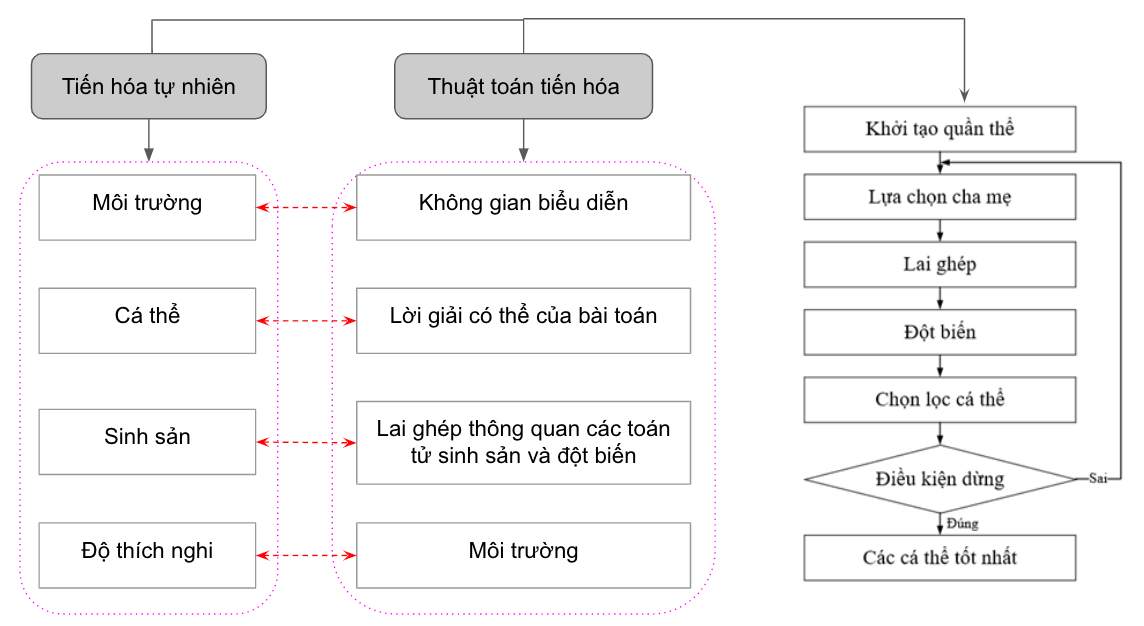
\includegraphics[width=0.85\linewidth]{ea_.png}}
    \caption{Tổng quan và các bước trong thuật toán tiến hóa}
    \label{fig:ea}
\end{figure}
\subsubsection{Khởi tạo}
 Quá trình khởi tạo - hay còn gọi là quá trình \textit{initialization} là quá trình khởi tạo một quần thể cho thế hệ đầu tiên. Đối với các bài toán tối ưu hóa liên tục, việc khởi tạo hầu hết được thực hiện theo cách ngẫu nhiên, chọn giá trị cho véc-tơ giải pháp trên một không gian nghiệm giới hạn. Với nhiều bài toán, thay vì lựa chọn một cách ngẫu nhiên, ta có thể dựa vào kết quả của một thuật toán tối ưu khác dựa vào một vài tri thức đã biết hoặc kinh nghiệm. Cách làm này có thể làm tăng tốc EA nhưng nó cũng là nguyên nhân gây ra sự đa dạng hóa thấp đi của lời giải vì quần thể được chọn đã rất giống lời giải so với lần chạy thực nghiệm trong thuật toán trước.
 Cách tiếp cận tốt nhất trong việc đưa ra quần thể đầu tiên có lẽ là nên nghiên cứu kỹ về các thuộc tính của vấn đề cần giải quyết bởi EA, sau đó chọn những thuộc tính mà ta quan tâm. Ví dụ, quần thể với mạng neural nhân tạo (thuật ngữ gốc: \emph{Artificial Neural Network - ANN}) có thể được khởi tạo bởi sơ đồ glorot ngẫu nhiên. \cite{glorot2010understanding}
 \subsubsection{Lựa chọn}
 Quá trình lựa chọn hay quá trình \emph{selection} có 2 kiểu khác nhau được thực hiện xuyên suốt trong mọi thế hệ đó là: lựa chọn để sinh sản và lựa chọn để thay thế trong quần thể. Lựa chọn để sinh sản được lấy cảm hứng từ tiến hóa trong sinh học, khi chỉ có những cá thể tốt nhất, khả năng sống sót cao nhất mới có thể truyền những yếu tố, đặc tính trong vật liệu di truyền của nó đến thế hệ con cháu. Giống như vậy, quy trình lựa chọn thay thế cũng giống như thực tế khi chỉ có những con cái khỏe mạnh với những đặc điểm tốt được thừa hưởng bởi bố mẹ mới có thể sống sót đến thế hệ tiếp theo. 
%  Nhưng thế nào là cá thể có đặc tính tốt, có khả năng sống sót cao? Tùy vào mỗi trường hợp khác nhau, yếu tố này sẽ thay đổi tuy nhiên dưới đây tôi xin trình bày một số phương pháp \emph{lựa chọn} trực tiếp liên quan đến đồ án này:
 
%  \begin{enumerate}
%  \item \textbf{Uniform selection:} Một cá thể được lựa chọn một cách ngẫu nhiên. Đây là hình thức chọn lọc yếu nhất vì không có điều kiện chọn lọc gì, áp lực chọn lọc thấp. Ngay cả những cá thể yếu nhất vẫn có những cơ hội bình đẳng được lựa chọn để tái sản xuất và di truyền đặc tính đến thế hệ tiếp theo so với những cá thể tốt nhất. Đây là một ví dụ dựa trên cách chọn lọc bình đẳng tuy nhiên cách này hầu như không được sử dụng.
%  \item \textbf{Fitness-proportional selection:} Giả sử rằng tất cả những giá trị fitness của hàm mục tiêu có giá trị dương. Một cá thể $x$ trong quần thể của thế hệ hiện tại $P$ có thể được chọn với xác suất $\frac{f(x)}{\sum_{u \in P}{f(u)}}$. Thay vì lựa chọn ngẫu nhiên như phương pháp \emph{uniform selection}, hình thức nãy sẽ đặt ra một độ đo để thực hiện chọn lọc. Tuy nhiên cách tiếp cận này lại phụ thuộc lớn vào những giá trị tốt fitness của hàm mục tiêu. Ví dụ: Nếu sự khác biệt giữa giá trị fitness trong dân số là quá lớn thì các cá thể có fitness cao nhất sẽ luôn được ưu tiên lựa chọn. Điều này sẽ làm ảnh hưởng đến sự đa dạng của quần thể hiện tại, và dẫn đến EA không thể khám phá ra khu vực thiết yếu trong không gian tìm kiếm. Tuy nhiên nếu các giá trị fitness của các cá thể là tương đương thì phương pháp này sẽ trở nên tương tự phương pháp \emph{uniform selection}. Thông thường trong những thế hệ đầu của EA trong việc giải quyết bài toán tối ưu hóa liên tục, giá trị fitness còn thấp nên sự khác biệt lớn giữa các cá thể sẽ mang tính quyết định. Các thế hệ sau đó, khi giá trị fitness của từng cá thể trong quần thể cao hơn, sự chênh lệch giữa chúng giảm dần, cơ chế lựa chọn sẽ dần trở thành tương tự \emph{uniform selection}. Hiện tượng này sẽ dần đến giảm hiệu quả trong quá trình lựa chọn và để giải quyết vấn đề này tôi sẽ giới thiệu phương pháp \emph{rank selection} như dưới đây.
%  \item \textbf{Rank selection:} Thay vì trực tiếp sử dụng fitness, kĩ thuật này sẽ thực hiện sắp xếp rank theo thứ tự giảm dần của fitness. Bằng phương pháp này, việc phụ thuộc vào những giá trị cụ thể của fitness bị loại bỏ. Việc lặp lại quá trình của \emph{fitness-proportional selection} dẫn đến trở về quá trình \emph{uniform selection} sẽ không xảy ra. Phương pháp này thường xuyên được sử dụng, áp dụng. Đặc biệt là thuật toán tối ưu hóa đa nhiệm hiện đại cũng áp dụng \emph{rank selection} để làm cơ sở trong việc tạo áp lực chọn lọc trong quá trình cải tiến nhiều nhiệm vụ của mình.
%  \end{enumerate}
 
 \subsubsection{Lai ghép}
Quá trình lai ghép (thuật ngữ gốc: \emph{crossover}) nhằm mục đích lấy những đặc điểm tốt của 2 hay nhiều cá thể cha mẹ để tạo ra những cá thể con cái có chất lượng cao hơn, mang một phần đặc tính di truyền của bố mẹ. Con cái được sinh ra có một phần sẽ giống với bố mẹ chúng và có thể khai thác được những gì mà bố mẹ chúng đã biết. Đồ án sẽ giới thiệu một số cơ chế lai ghép liên quan đến phạm vi nghiên cứu:

\begin{enumerate}
    \item \textbf{One point crossover:} Đầu tiên 2 cá thể $p_1$ và $p_2$ trong quần thể cha mẹ được chọn. Sau đó ta sẽ chọn hệ số chia cắt index $i \in \{1, ..., n-1\}$, Sau đó 2 cha mẹ sẽ hoán đổi tại vị trí $i$ giống như trong hình \ref{fig:introduction:one_point}.
    \begin{figure}[ht]
        \centering
        \fbox{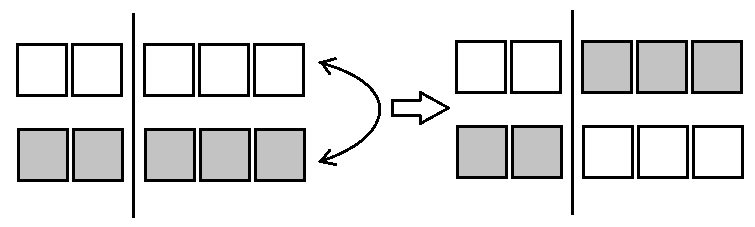
\includegraphics[width=0.8\linewidth]{images/one_point.png}}
        \caption{Kỹ thuật one point crossover}
        \label{fig:introduction:one_point}
    \end{figure}
    \item \textbf{Uniform crossover:} Đầu tiên 2 cá thể $p_1$ và $p_2$ trong quần thể cha mẹ được chọn. Sau đó với mỗi chiều $i \in \{1, ..., n\}$ giá trị của con cái $x_i$ sẽ là bản được sao chép từ một trong các cha mẹ của chúng. Quyết định cha mẹ nào sẽ được chọn để sao chép sẽ được tạo ra độc lập bởi tại mỗi chiều với xác suất bằng $\frac{1}{2}$.
    \item \textbf{Simulated binary crossover - SBX:} SBX \cite{deb1995simulated} \cite{deb94simulated} là một kỹ thuật lai ghép kết hợp tham số là số thực thường được sử dụng trong EA. Trong đó, một lời giải bao gồm các giá trị số thực liên tục cần được chuyển sang dạng nhị phân để áp dụng kĩ thuật one point crossover với các lời giải khác. Tuy nhiên thay vì sử dụng cách này, SBX được thiết kế để chỉ sử dụng các phân phối xác suất. Các bước của SBX được mô tả như dưới đây:
        \begin{enumerate}
            \item Chọn cặp bố mẹ $p_1$ và $p_2$ để lai ghép ($p_1, p_2 \in \text{ khoảng } [0, 1] ^ n$)
            \item Khởi tạo ngẫu nhiên véc-tơ $u \sim U(0,1)^n$
            \item Khởi tạo đặc tính chung $cf$
                 \[
                    cf=\left\{
                        \begin{array}{ll}
                            2*u_i^{\frac{1}{\alpha + 1}} \text{ if } u_i > 0.5\\
                            2*(1-u_i)^{\frac{-1}{\alpha + 1}} \text{ if } u_i \leq 0.5\\
                        \end{array}
                    \right.
                  \]
                Tham số $\alpha$ là chỉ số của phân phối SBX, thường có giá trị từ $2$ đến $5$. Hình \ref{fig:introduction:sbx} biểu thị mối quan hệ giữa của tập con cái và cha mẹ khi được sinh ra bởi các phân phối SBX khác nhau. Chỉ số phân phối nhỏ hơn sẽ khuyến khích sự khám phá vì con cái tương đối xa cha mẹ của chúng.
            \item Tạo 2 con
                 \[
                     \begin{array}{ll}
                        c_1 = \frac{1}{2} (1 + cf) * p_1 + (1 - cf) * p_2\\
                        c_2 = \frac{1}{2} (1 + cf) * p_2 + (1 - cf) * p_1
                    \end{array}
                  \]
        \end{enumerate}
        \begin{figure}[ht]
            \centering
            \fbox{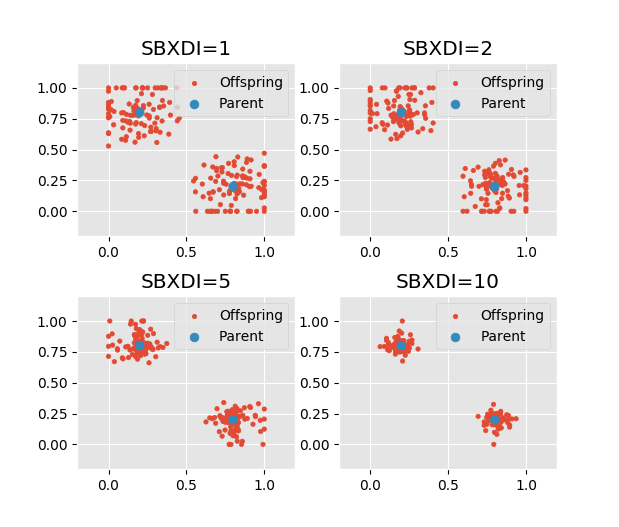
\includegraphics[width=0.8\linewidth]{sbx.png}}
            \caption{Mô phỏng 100 con cái được tạo ra từ thuật toán lai ghép SBX với các chỉ số phân phối khác nhau}
            \label{fig:introduction:sbx}
        \end{figure}
\end{enumerate}

\subsubsection{Đột biến}
Ngược lại với lai ghép, mục đích của đột biến hay còn gọi là \emph{mutation} là để khám phá ra thêm không gian tìm kiếm. lai ghép khai thác, tái sử dụng những giá trị, thông tin đã tồn tại trong một tập các cá thể, bởi vậy quần thể được sinh ra sẽ ngày càng có độ đa dạng giảm đi. Do đó đột biến sẽ tạo ra những thay đổi nhỏ trong các giải pháp thu được, có thể hiểu một cách đơn giản như ta sẽ đưa thêm các vật liệu di truyền mới vào các nhóm gen đã có để tăng sự đa dạng của quần thể. Đột biến sẽ không tạo ra thay đổi lớn trong cá thể gốc bởi vì nó sẽ phá vỡ cấu trúc đã được hình thành trong giải pháp của quần thể cha mẹ, những con cái được chọn để đột biến là ngẫu nhiên mà không tuân theo nguyên tắc cụ thể nào.

Kết hợp quá trình lai ghép và đột biến sẽ giúp tinh chỉnh các tham số của lời giải nhằm mục đích cân bằng giữa việc khai thác và khám phá giúp EA tìm ra những giải pháp tối ưu hơn. Trong các phương pháp đột biến thì Gaussian mutation là một trong những kĩ thuật đột biến phổ biến nhất trong tối ưu hóa liên tục. Trong kĩ thuật này, các con cái là $y \in \mathbb{R}^n$ sẽ được xây dựng bằng cách sử dụng giải pháp của bố mẹ $x \in \mathbb{R} ^ n$ thêm với một lượng nhiễu nhỏ $m \in \mathbb{R}^n$. Giá trị nhiễu $m$ này sẽ phải đủ nhỏ để tuân theo nguyên tắc chỉ gây ra một chút thay đổi nhỏ cho tập con cái. Giá trị nhiễu $m \sim \mathbb{N}(0, I*\sigma^2)$ với $\sigma$ là độ lệch chuẩn nhỏ.